\chapter{Neural network}\label{chap:nn}

\section{Selection of Neural Network Architecture}

In light of the temporal nature of our data, we required a neural network
architecture capable of handling sequential data. Various neural network
architectures cater to this requirement. For instance, \gls{rnn} which use
outputs from previous steps as inputs for subsequent steps, excel at handling
sequential data. This trait enables \gls{rnn}s to retain information from
previous steps, a characteristic beneficial for time series analysis.

However, one downside of RNNs is the vanishing gradients problem, wherein they
tend to forget information from earlier stages in the sequence. Various
\gls{rnn} variations, such as \gls{lstm} \cite{lstm:1997} and \gls{gru}
\cite{gru:2014}, have been designed to mitigate this issue.

On the other hand, Transformer networks \cite{attention2017}, a more recent
introduction to the world of neural networks, have seen significant success in
natural language processing. These networks utilize attention mechanisms,
allowing them to concentrate on specific portions of an input sequence. While
useful for time series analysis, the major drawback of Transformer networks is
their need for vast amounts of training data\todo[]{citation needed} --- a
requirement we couldn't fulfill in this case.

Upon weighing these factors, we decided to adopt a neural network architecture
utilizing an \gls{lstm}.

\section{Neural network architecture}

Utilizing the PyTorch library, we built our custom \gls{lstm}-based neural
network architecture. PyTorch's \texttt{pack\_padded\_sequence} and
\texttt{pad\_packed\_sequence} functions were used to pack and unpack sequences
into single tensors, accommodating patients with varying numbers of sessions.
An additional tensor of \textit{lengths} was used to facilitate the input of
the packed sequences into the \gls{lstm}, which consequently ignored the values
beyond the length of the sequence.

\begin{figure}
    \centering
    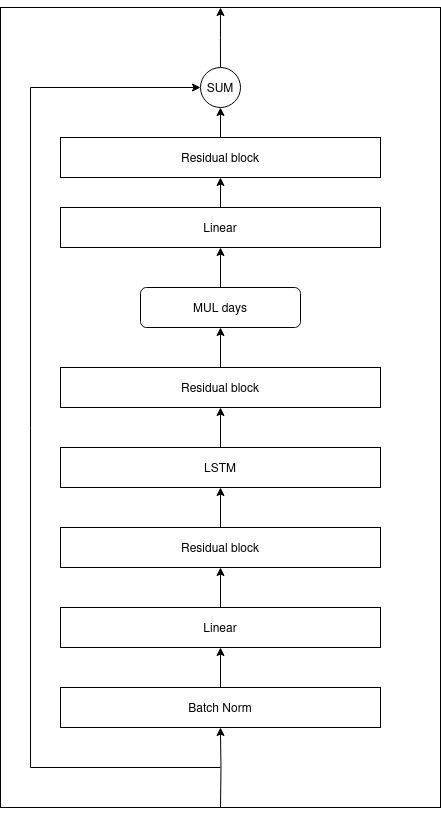
\includegraphics[width=8cm]{files/nn_diagram}
    \caption{Diagram of the implemented \gls{lstm}-based neural network architecture}
\end{figure}

\subsection{Variability in the dates of the sessions}

The dataset's sessions are not uniformly spaced in time, varying from a few
days to several months apart. This is a problem for neural networks, since they
work best with uniformly spaced data. To solve this problem, we decided to make
the neural network predict the daily change instead.

This was accomplished by adding a residual connection between the input and the
output of the neural network, and multiplying the output by the number of days
until the next session. This way, the neural network can learn to predict the
daily change, and the output is scaled to the number of days until the next
session.
\section{Training and Optimization}

During the training phase, the neural network receives input in the form of a
tensor with a shape of $(\text{batch size}, \text{max sequence length},
    \text{number of features})$, a tensor with a shape of $(\text{batch size}, 1)$
containing the length of the current sequence, and a scalar representing the
number of days until the next session. It then generates a tensor of shape
(\text{batch size}, \text{max sequence length}, \text{number of features}) that
contains the predicted values for the next session.

The neural network takes the following inputs:

\begin{itemize}
    \item A tensor of shape $(\text{batch size}, \text{max sequence length}, \text{number
                  of features})$.
    \item A tensor of shape $(\text{batch size}, 1)$ containing the length of the current
          sequence.
    \item A scalar representing the number of days until the next session.
\end{itemize}

The neural network returns:

\begin{itemize}
    \item A tensor of shape $(\text{batch size}, \text{max sequence length}, \text{number
                  of features})$ that contains the predicted values for the next session.
\end{itemize}

To construct the input features, we concatenate the $\beta$ parameters of the
\gls{smpl} model with the patient's height, weight, and age.

We also experimented with including body fat percentage and muscle mass
percentage, but the results did not show improvement, so we decided to exclude
them in order to avoid overfitting.

We utilized the AdamW optimizer with a variable learning rate and weight decay,
along with \gls{mse} loss as the objective function.

\subsection{Hyperparameter tuning}

We performed a grid search to find the optimal hyperparameters for our model.
The hyperparameters we tuned were the number of layers in the input, \gls{lstm}
and output, the number of hidden units in the \gls{lstm} and the weight decay.

The final hyperparameters we used are shown in
Table~\ref{tab:final-hyperparameters}.

\begin{table}[h]
    \centering
    \begin{tabular}{l c c}
        \toprule
        \textbf{Hyperparameter}                  & \textbf{Value} \\
        \midrule
        Number of layers in the input            & 4              \\
        Number of layers in the \gls{lstm}       & 4              \\
        Number of layers in the output           & 4              \\
        Number of hidden units in the \gls{lstm} & 32             \\
        Weight decay                             & 0.001          \\
        \bottomrule
    \end{tabular}
    \caption{Final hyperparameters used for the neural network}
    \label{tab:final-hyperparameters}
\end{table}

\section{Results}

While a more detailed analysis of the results will be presented in the next
chapter, we provide some examples of our model's predictions.

Figure \ref{fig:predicted-betas} displays the shape parameters for a patient
alongside the model's prediction.

\begin{figure}[h]
    \centering
    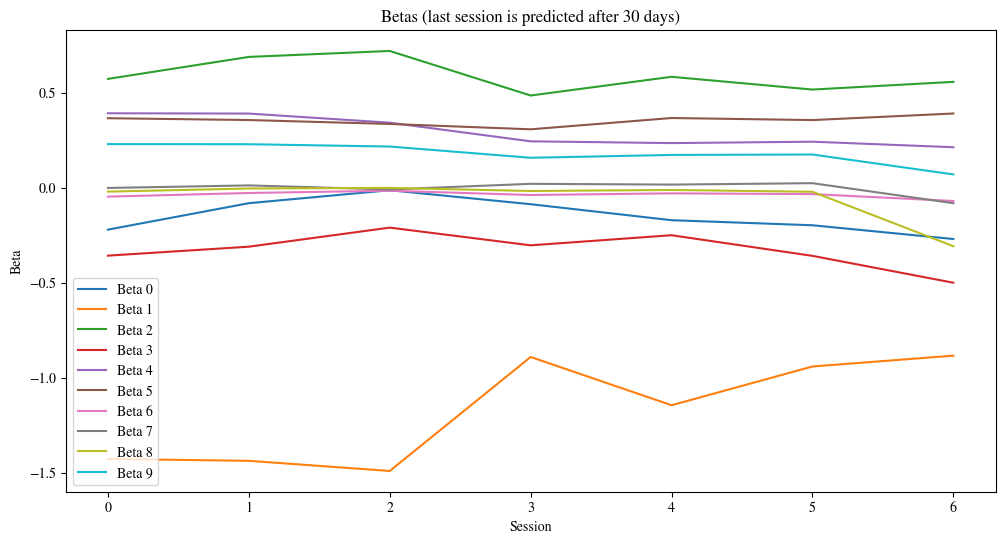
\includegraphics[width=\textwidth]{files/predicted_betas}
    \caption{Shape parameters for a patient and the model's prediction.}
    \label{fig:predicted-betas}
\end{figure}

Figure \ref{fig:patient-body-model} illustrates the reconstructed 3D model of a
patient's body, showcasing images from multiple sessions. The final image in
the sequence represents the model's prediction after one month from the last
session, with a total of 74 days between the first and last session.

\begin{figure}[h]
    \centering
    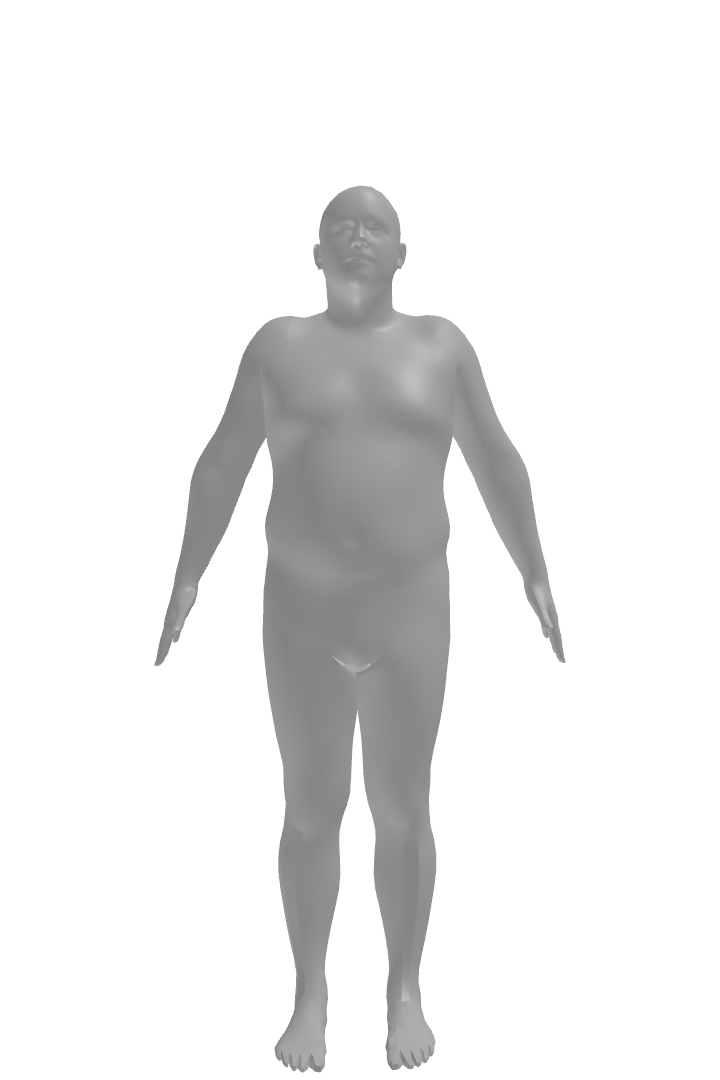
\includegraphics[width=120pt]{files/patient_2/2_6}
    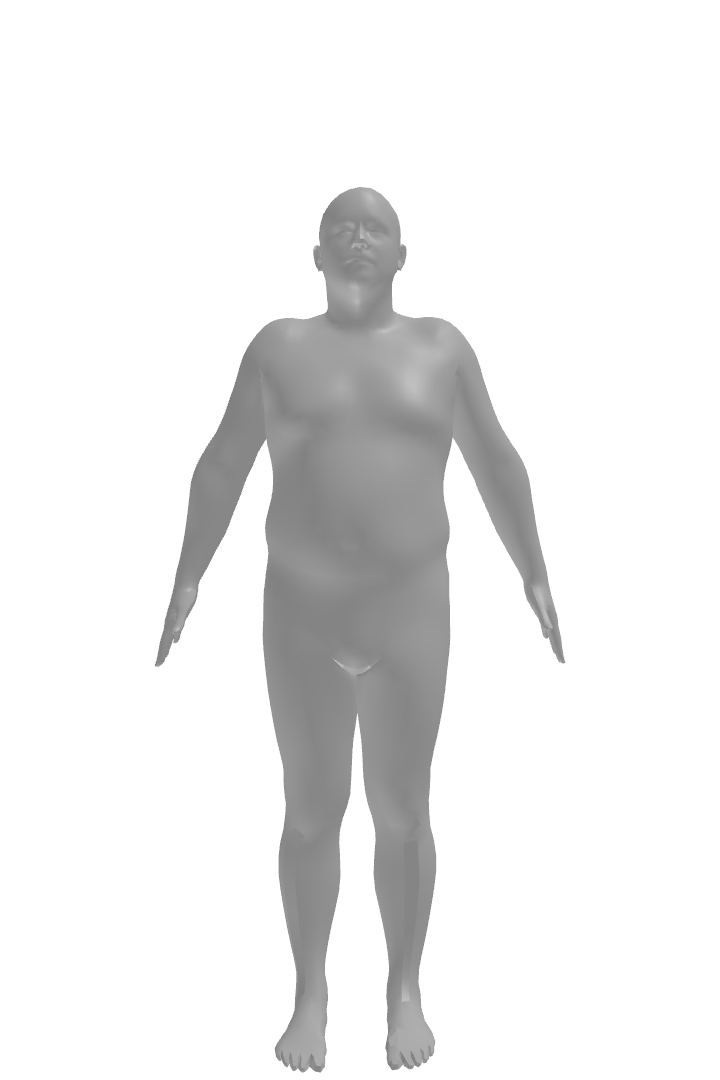
\includegraphics[width=120pt]{files/patient_2/2_7}
    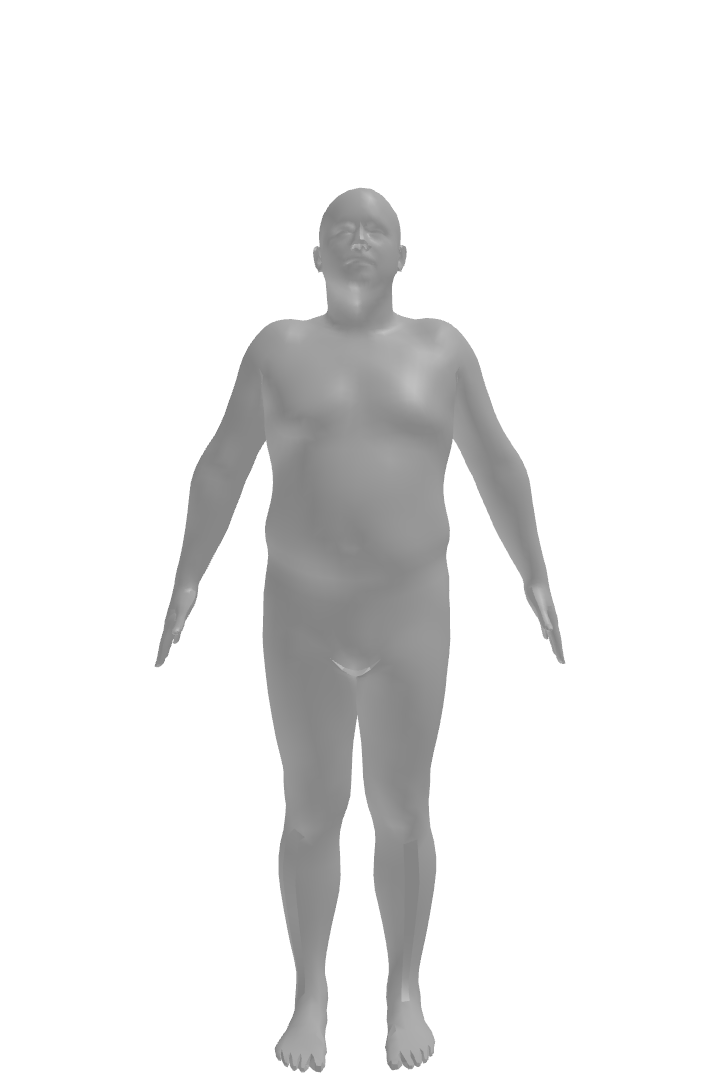
\includegraphics[width=120pt]{files/patient_2/2_8}
    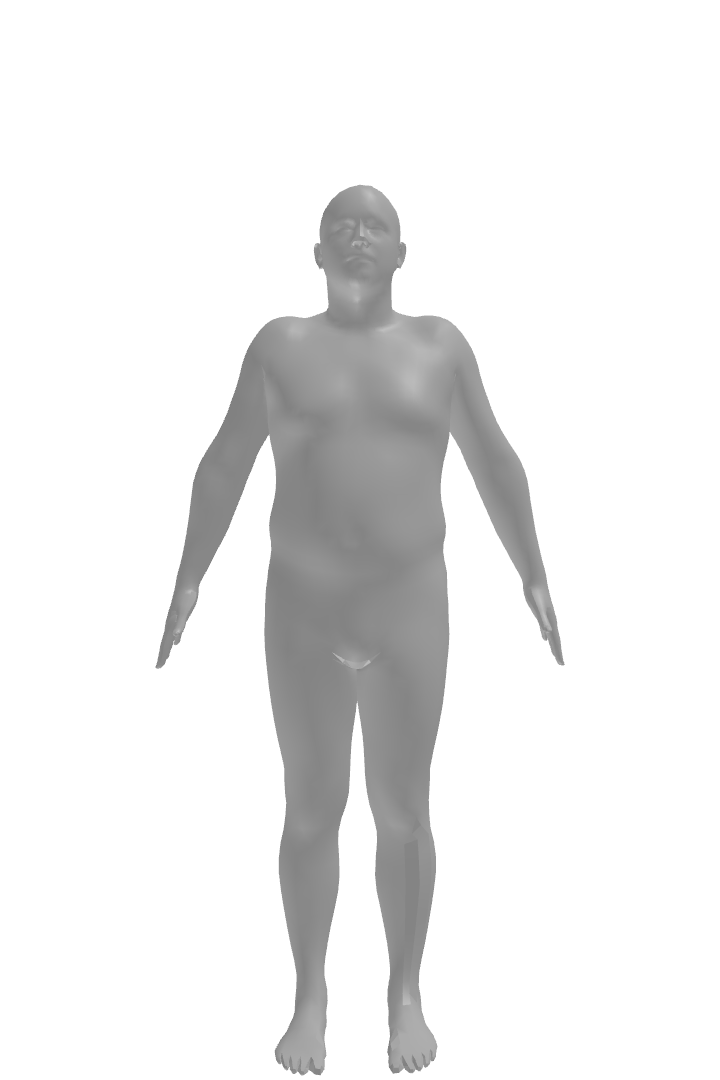
\includegraphics[width=120pt]{files/patient_2/2_9}
    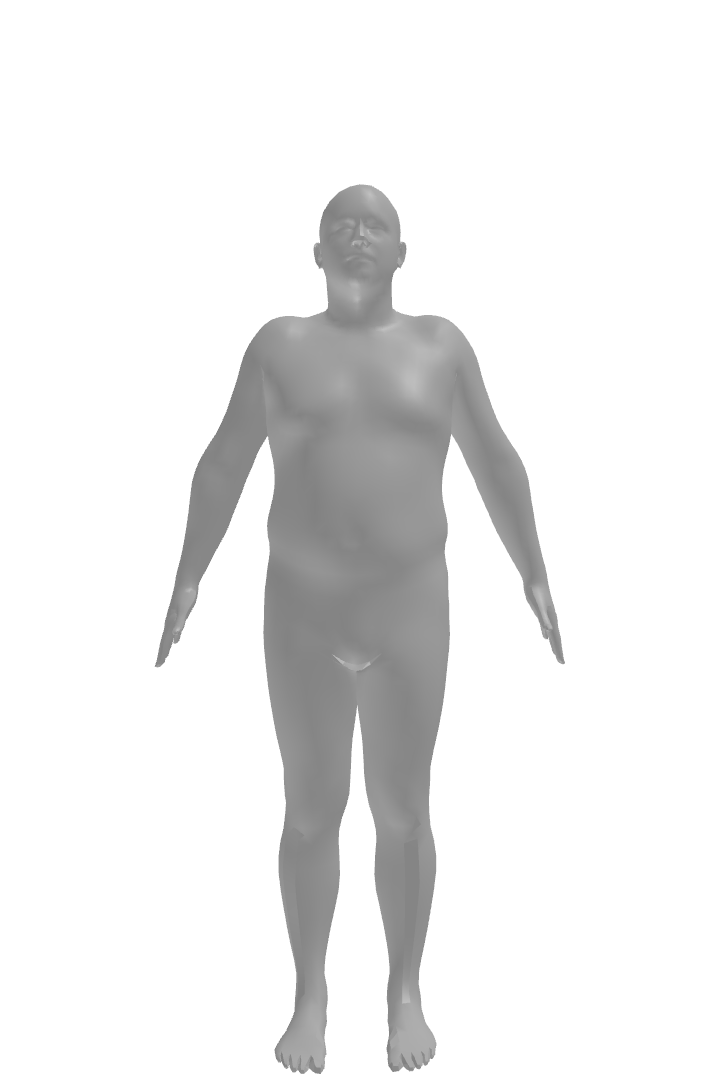
\includegraphics[width=120pt]{files/patient_2/2_10}
    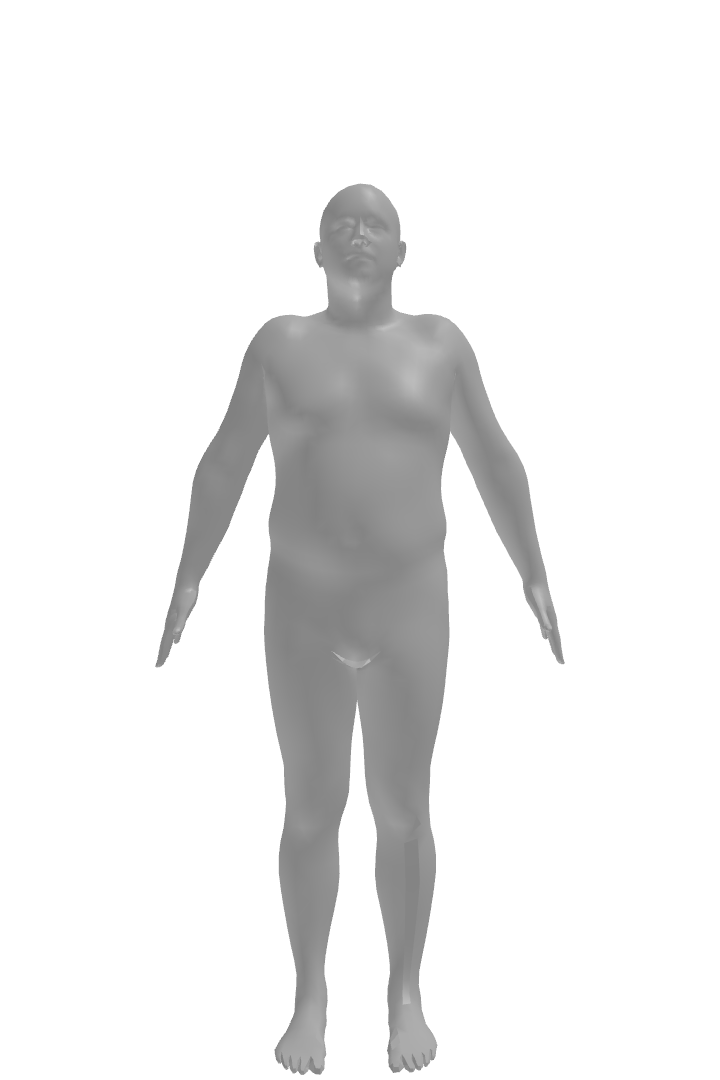
\includegraphics[width=120pt]{files/patient_2/2_11}
    \linebreak
    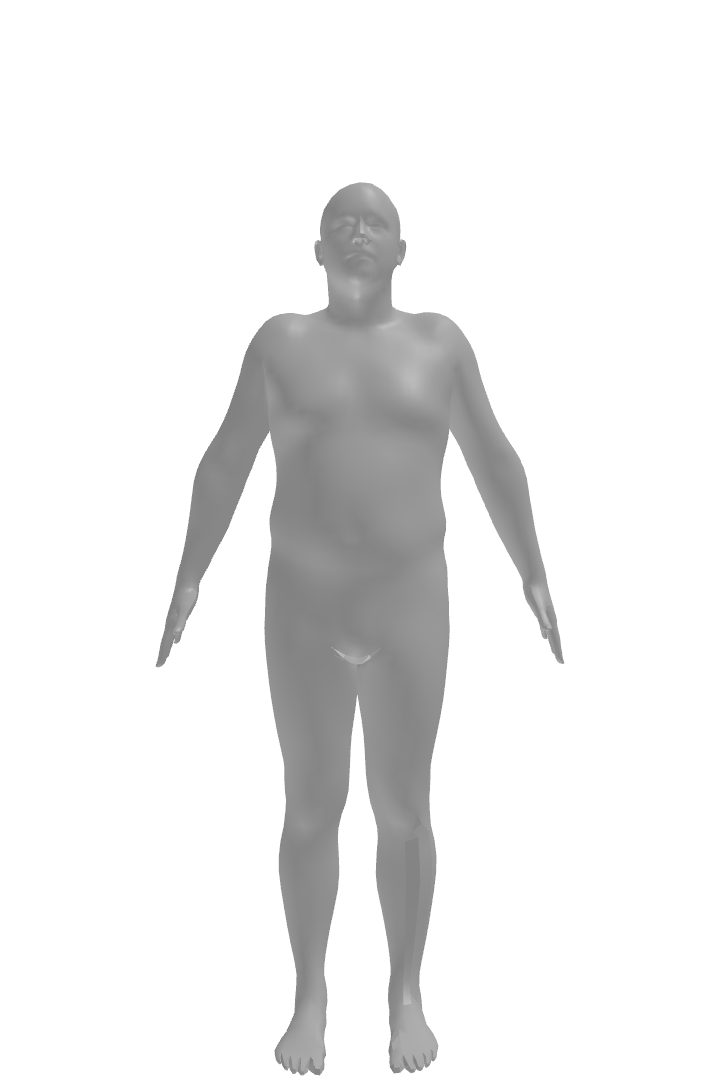
\includegraphics[width=120pt]{files/patient_2/2_predicted}
    \caption[Reconstructed 3D model of the patient's body]{Reconstructed 3D model of the patient's body. The last image is the model's prediction after one month from the last session. There are a total of 74 days between the first and last session.}
    \label{fig:patient-body-model}
\end{figure}

The results obtained provide an initial understanding of the model's
performance and will be further examined and discussed in the subsequent
chapter.